% Theorie: Physikalische Grundlagen von Versuch/Messverfahren, Gleichungen ohne Herleitung knapp erklären
\section[Theorie]{Theorie \textnormal{\cite{photo}}}
\label{sec:theorie}

\subsection{Eigenschaften von Licht}

\subsection{Lichtelektrischer Effekt}

\begin{figure}[H]
	\centering
	\hspace{4ex}
	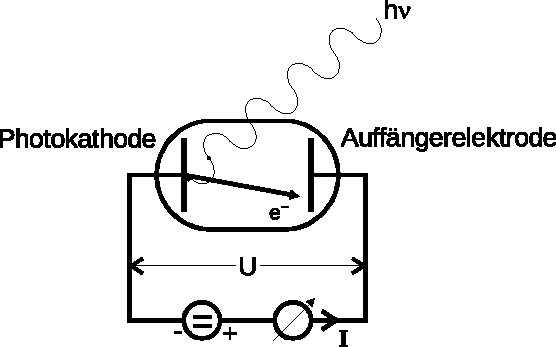
\includegraphics[width=0.5\linewidth]{content/grafik/prinzip.pdf}
	\caption{}
	\label{fig:prinzip}
\end{figure}

\subsection{Grundlagen der Apparatur}

\begin{figure}[H]
	\centering
	\hspace{12.5ex}
	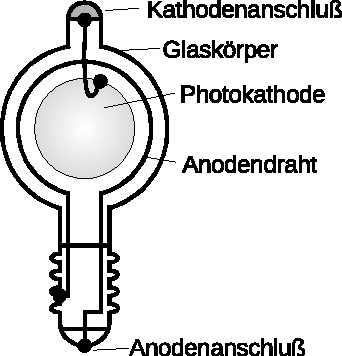
\includegraphics[width=0.3\linewidth]{content/grafik/photozelle.pdf}
	\caption{}
	\label{fig:photozelle}
\end{figure}

\begin{figure}[H]
	\centering
	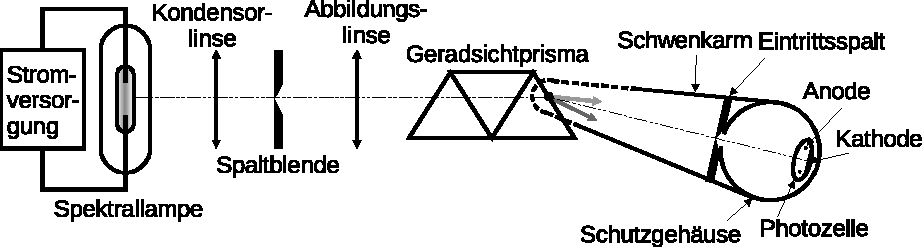
\includegraphics[width=0.8\linewidth]{content/grafik/optik.pdf}
	\caption{}
	\label{fig:optik}
\end{figure}

\begin{figure}[H]
	\centering
	\hspace{6ex}
	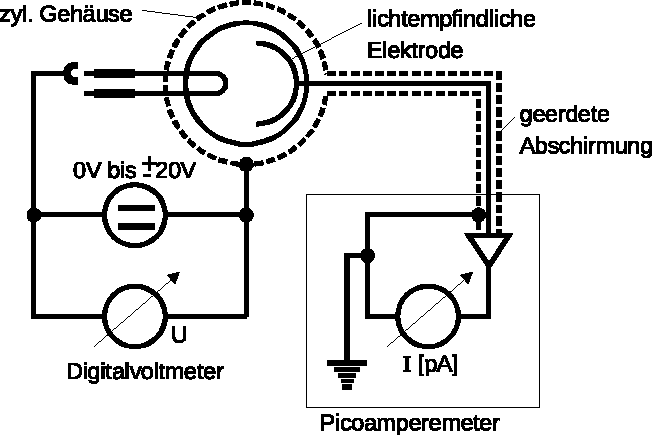
\includegraphics[width=0.6\linewidth]{content/grafik/schaltbild.pdf}
	\caption{}
	\label{fig:schaltbild}
\end{figure}

\begin{figure}[H]
	\centering
	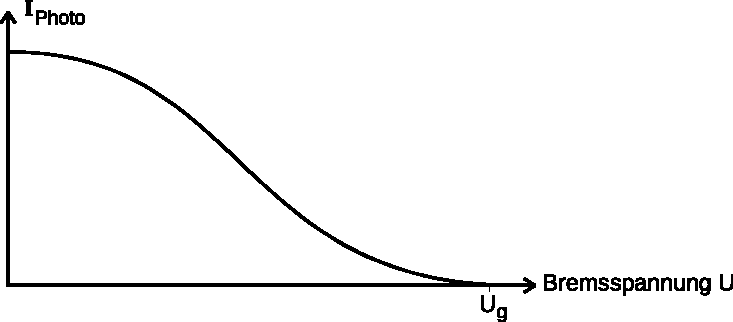
\includegraphics[width=0.7\linewidth]{content/grafik/kurve.pdf}
	\caption{}
	\label{fig:kurve}
\end{figure}

\begin{figure}[H]
	\centering
	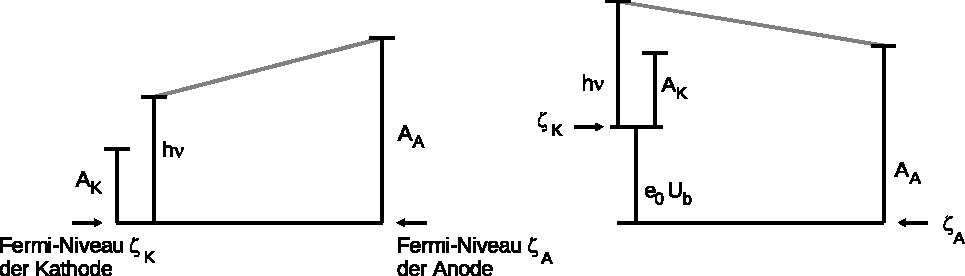
\includegraphics[width=0.9\linewidth]{content/grafik/potential.pdf}
	\caption{}
	\label{fig:potential}
\end{figure}

